\chapter{Generating random performance tableaux}
\label{sec:6}

\abstract*{ The Chapter describes the \Digraph resources for generating random multiple criteria performance tableaux. These random performance tableaux instances, mainly meant for illustration and training purposes, are serving the preparation and illustration of the \emph{Algorithmic Decision Theory} Course lectures. The random generators propose several useful models, like a \emph{Cost-Benefit} tableau, a three Objectives --\emph{economic}, \emph{societal} and \emph{environmental}-- tableau, and evetually an \emph{academic} performance tableau.}

\abstract{ The Chapter describes the \Digraph resources for generating random multiple criteria performance tableaux. These random performance tableaux instances, mainly meant for illustration and training purposes, are serving the preparation and illustration of the \emph{Algorithmic Decision Theory} Course lectures. The random generators propose several useful models, like a \emph{Cost-Benefit} tableau, a three Objectives --\emph{economic}, \emph{societal} and \emph{environmental}-- tableau, and evetually an \emph{academic} performance tableau.}

\section{Introduction}
\label{sec:6.1}

The {\tt randomPerfTabs} module provides several constructors for generating random performance tableaux models of different kind, mainly for the purpose of testing implemented methods and tools presented and discussed in the Algorithmic Decision Theory course lectures at the University of Luxembourg. This chapter introduces the most useful models.

The simplest model, called \emph{RandomPerformanceTableau}, generates a set of $n$ decision actions, a set of $m$ real-valued performance criteria, ranging by default from $0.0$ to $100.0$, associated with default discrimination thresholds: $2.5$ (ind.), $5.0$ (pref.) and $60.0$ (veto). The generated performances are Beta(2,2) distributed on each measurement scale.

One of the most useful models, called \emph{RandomCBPerformanceTableau}, proposes a performance tableau involving two decision objectives, named \emph{Costs} (to be minimized) respectively \emph{Benefits} (to be maximized); its purpose being to generate more or less contradictory performances on these two, usually conflicting, objectives. \emph{Low costs} will randomly be coupled with \emph{low benefits}, whereas \emph{high costs} will randomly be coupled with \emph{high benefits}.

Many public policy decision problems involve three often conflicting decision objectives taking into account \emph{economical}, \emph{societal} as well as \emph{environmental} aspects. For this type of performance tableau model, we provide a specific model, called \emph{Random3ObjectivesPerformanceTableau}.

Deciding which students, based on the grades obtained in a number of examinations, validate or not their academic studies, is the genuine decision practice of universities and academies. To thouroughly study these kind of decision problems, we provide a corresponding performance tableau model, called \emph{RandomAcademicPerformanceTableau}, which gathers grades obtained by a given number of students in a given number of weighted courses.    

In order to study aggregation of election results (see Chapter \ref{sec:7}) in the context of bipolar-valued outranking digraphs, we provide furthermore a specific performance tableau model called \emph{RandomRankPerformanceTableau} which provides ranks (linearly ordered performances without ties) of a given number of election candidates (decision actions) for a given number of weighted voters (performance criteria).
 
\section{Random standard performance tableaux}
\label{sec:6.2}
    
The {\tt RandomPerformanceTableau} class\index{RandomPerformanceTableau@\texttt{RandomPerformanceTableau} class}, the simplest of the kind, specializes the generic {\tt PerformanceTableau} class, and takes the following parameters:
\begin{itemize}[leftmargin=0.5cm,rightmargin=0.5cm]
\item \texttt{numberOfActions} := number of decision actions.
\item \texttt{numberOfCriteria} := number of performance criteria.
\item \texttt{weightDistribution} := \\
   \texttt{'random'} (default) $|$ \texttt{'fixed'} $|$ \texttt{'equisignificant'}:
      \begin{itemize}[rightmargin=1cm]
         \item If \texttt{'random'}, weights are uniformly selected randomly from the given weight scale;
         \item If \texttt{'fixed'}, the weightScale must provided a corresponding weights distribution;
         \item If \texttt{'equisignificant'}, all criterion weights are put to unity.
      \end{itemize}
\item \texttt{weightScale} := \texttt{[Min,Max]} (default =(1, \texttt{numberOfCriteria}).
\item \texttt{IntegerWeights} := \texttt{True} (default) $|$ \texttt{False} (normalized to proportions of $1.0$).
\item \texttt{commonScale} := \texttt{[a,b]}; common performance measuring scales (default = $[0.0,100.0]$)
\item \texttt{commonThresholds} := [(\texttt{q0}, \texttt{q1}), (\texttt{p0}, \texttt{p1}), (\texttt{v0}, \texttt{v1})]; indifference($q$), preference ($p$) and considerable performance difference ($v$) discrimination thresholds. For each threshold type $x \in \{q,p,v\}$, the float $x0$ value represents a \emph{constant percentage} of the common scale and the float $x1$ value a \emph{proportional value} of the actual performance measure. Default values are $[(2.5.0,0.0), (5.0,0.0), (60.0,0,0)]$. 
\item \texttt{commonMode} := common random distribution of random performance measurements:
      \begin{itemize}[rightmargin=1cm]
         \item (\texttt{'beta'}, \texttt{None} (default setting), ($\alpha$, $\beta$)), a beta generator with default $\alpha=2$ and $\beta=2$ parameters.
         \item  (\texttt{'uniform'}, \texttt{None}, \texttt{None}), uniformly distributed float values on the given common scales' range \texttt{[Min, Max]};
         \item (\texttt{'normal'}, $\mu$, $\sigma$), truncated Gaussian distribution, by default $\mu = (b-a)/2$ and $\sigma = (b-a)/4$;
         \item (\texttt{'triangular'}, \emph{mode}, \emph{repartition}), generalized triangular distribution with a probability repartition parameter specifying the probability mass accumulated until the mode value. By default, \emph{mode} = $(b-a)/2$ and \texttt{repartition} = $0.5$.
      \end{itemize}
\item \texttt{valueDigits} := \texttt{integer}, precision of performance measurements (2 decimal digits by default).
\item \texttt{missingDataProbability} := $0.0 \leq \mathtt{float} \leq 1.0$ ; probability of missing performance evaluation on a criterion for an alternative (default $0.025$).
\item \texttt{NA} := \texttt{Decimal} (default = $-999$); missing data symbol. 
\end{itemize} 

\noindent \textbf{Code example:}
\begin{lstlisting}[caption={Generating a random performance tableau},label=list:6.1]
>>> from randomPerfTabs import RandomPerformanceTableau
>>> t = RandomPerformanceTableau(numberOfActions=21,\
...                 numberOfCriteria=13,seed=100)
>>> t.actions
  {'a01': {
    'comment': 'RandomPerformanceTableau() generated.',
    'name': 'random decision action'
    },
   'a02': { ... },
    ...
   }
>>> t.criteria
  {'g01': {
    'thresholds': {
      'ind' : (Decimal('10.0'), Decimal('0.0')),
      'veto': (Decimal('80.0'), Decimal('0.0')),
      'pref': (Decimal('20.0'), Decimal('0.0'))},
    'scale': [0.0, 100.0],
    'weight': Decimal('1'),
    'name': 'RandomPerformanceTableau() instance',
    'comment': "Arguments: weightDistribution=random;
                           weightScale=(1, 1);
                           commonMode=None"
    },
   'g02':  { ... },
   ...
  }
>>> t.evaluation
  {'g01': {'a01': Decimal('15.17'),
           'a02': Decimal('44.51'),
           'a03': Decimal('-999'), # missing evaluation
       ...  },
   ...
 }
>>> t.showHTMLPerformanceTableau()
\end{lstlisting}
\begin{figure}[h]
%\sidecaption
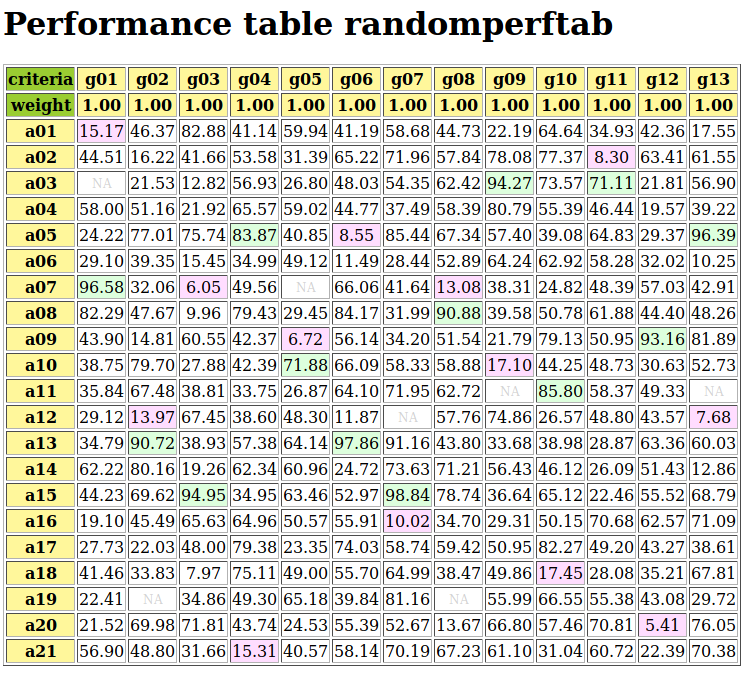
\includegraphics[width=11cm]{Figures/randomPerfTab1.png}
\caption{Browser view on random performance tableau instance}
\label{fig:6.1}       % Give a unique label
\end{figure}
Best and worst performance on each criterion are marked in \emph{light green}, respectively in \emph{light red}. Notice that missing (\texttt{NA}) evaluation are registered in a performance tableau by default as \texttt{Decimal('-999')} value (see Listing \ref{list:6.1} Line 24).	    
\section{Random Cost-Benefit performance tableaux}
\label{sec:6.3}

We provide the \texttt{RandomCBPerformanceTableau} class\index{RandomCBPerformanceTableau@\texttt{RandomCBPerformanceTableau} class} for generating random \emph{Costs} versus \emph{Benefits} organized performance tableaux following the directives below:
\begin{itemize}[leftmargin=0.5cm,rightmargin=0.5cm]
\item We distinguish three types of decision actions: \emph{cheap}, \emph{neutral} and \emph{expensive} ones with an equal proportion of 1/3. We also distinguish two types of weighted criteria: \emph{Costs} criteria to be \emph{minimized}, and \emph{Benefits} criteria to be \emph{maximized}; in the proportions 1/3 respectively 2/3. 
\item  Random performances on each type of criteria  are drawn, either from an ordinal scale $[0;10]$, or from a cardinal scale $[0.0;100.0]$, following a parametric triangular law of mode: $30\%$ performance for cheap, $50\%$ for neutral, and $70\%$ performance for expensive decision actions, with constant probability repartition $0.5$ on each side of the respective mode. 
\item Costs criteria use mostly cardinal scales (3/4), whereas Benefits criteria use mostly ordinal scales (2/3). 
\item  The sum of weights of the Costs criteria by default equals the sum weights of the Benefits criteria: \texttt{weighDistribution} = 'equiobjectives'. 
\item On cardinal criteria, both of cost or of benefit type, we observe following constant preference discrimination quantiles: $5\%$ indifferent situations, $90\%$ strict preference situations, and $5\%$ veto situation. 
\end{itemize}

\textbf{Parameters}:
\begin{itemize}[leftmargin=0.5cm,rightmargin=0.5cm]
\item If \texttt{numberOfActions == None}, a uniform random number between 10 and 31 of \emph{cheap}, \emph{neutral} or \emph{advantageous} actions (equal 1/3 probability each type) actions is instantiated;
\item If \texttt{numberOfCriteria == None}, a uniform random number between 5 and 21 of cost or benefit criteria (1/3 respectively 2/3 probability) is instantiated;
\item \emph{weightDistribution} :=  \texttt{'equisignificant'} (default) $|$\\
  \texttt{'equiobjectives'} $|$ \texttt{'fixed'} $|$ \texttt{'random'};
\item default \texttt{weightScale} for 'random' weight distribution is\\ 1 - \texttt{numberOfCriteria};
\item All \emph{cardinal} criteria are evaluated with decimals between $0.0$ and $100.0$ whereas \emph{ordinal} criteria are evaluated with integers between 0 and 10.
\item \texttt{commonThresholds} is obsolete. Preference discrimination is specified as \emph{percentiles} of concerned performance differences (see below).
\item \texttt{commonPercentiles} := \texttt{\{'ind':5, 'pref':10, 'veto':95\}} are expressed in percents (reversed for vetoes), and only concern cardinal criteria.
\item \texttt{missingDataProbability} := $0.0 \leq \mathtt{float} \leq 1.0$ ; probability of missing performance evaluation on a criterion for an alternative (default $0.025$).
\item \texttt{NA} := \texttt{Decimal} (default = $-999$); missing data symbol. 
\end{itemize}

Minimal number of decision actions required is 3 ! 

\noindent \textbf{Example Python session}:
\begin{lstlisting}[caption={Generating a random Cost-Benefit performance tableau},label=list:6.2]
>>> from randomPerfTabs import\
...              RandomCBPerformanceTableau
>>> t = RandomCBPerformanceTableau(
...          numberOfActions=7,\
...          numberOfCriteria=5,\
...          weightDistribution='equiobjectives',\
...          commonPercentiles={'ind':0.05,
...                             'pref':0.10,\
                                'veto':0.95},\
...          seed=100)
>>> t.showActions()
  *----- show decision action --------------*
    key:  a1
      short name: a1c
      name:  random cheap decision action
    key:  a2
      short name: a2n
      name:  random neutral decision action
    ...
    key:  a7
      short name: a7a
      name:  random advantageous decision action
>>> t.showCriteria()
  *----  criteria -----*
   b1 'random ordinal benefit criterion'
    Scale = (0, 10)
    Weight = 3
    ...
   c1 'random cardinal cost criterion'
    Scale = (0.0, 100.0)
    Weight = 2 
    Threshold ind  :  1.76 + 0.00x ; percentile:  9.5
    Threshold pref :  2.16 + 0.00x ; percentile: 14.3
    Threshold veto : 73.19 + 0.00x ; percentile: 95.2
    ...}
\end{lstlisting}
In the example above, we may notice the three types of decision actions (see Listing \ref{list:6.2} Lines 10-20), as well as the two types (Lines 22-32) of criteria with either an \emph{ordinal} or a \emph{cardinal} performance measuring scale. In the latter case, by default about $5\%$ of the random performance differences will be below the \emph{indifference} and $10\%$ below the \emph{preference} discriminating threshold. About $5\%$ will be considered as \emph{considerably large}. More statistics about the generated performances may be inspected with the \texttt{showStatistics()} method.\index{showStatistics@\texttt{showStatistics()}}
\begin{lstlisting}
>>> t.showStatistics()
    *-------- Performance tableau summary statistics -------*
    Instance name      : randomCBperftab
    Actions            : 7
    Criteria           : 5
     Criterion name       : b1
       Criterion weight     : 3
       criterion scale    : 0.00 - 10.00
       mean evaluation    : 5.14
       standard deviation : 2.64
       maximal evaluation : 8.00
       quantile Q3 (x_75) : 8.00
       median evaluation  : 6.50
       quantile Q1 (x_25) : 3.50
       minimal evaluation : 1.00
       mean absolute difference      : 2.94
       standard difference deviation : 3.74
      ...
     Criterion name       : c1
       Criterion weight     : 2
       criterion scale    : -100.00 - 0.00
       mean evaluation    : -49.32
       standard deviation : 27.59
       maximal evaluation : 0.00
       quantile Q3 (x_75) : -27.51
       median evaluation  : -35.98
       quantile Q1 (x_25) : -54.02
       minimal evaluation : -91.87
       mean absolute difference      : 28.72
       standard difference deviation : 39.02
     ...
\end{lstlisting}

A heatmap view with 5 color levels gives the result shown in Fig.~\ref{fig:6.2}.
\begin{lstlisting}
>>> t.showHTMLPerformanceHeatmap(colorLevels=5,\
...        rankingRule=None,\
...        pageTitle='Random Cost-Benefit Performance Tableau')
 \end{lstlisting}
\begin{figure}[h]
%\sidecaption
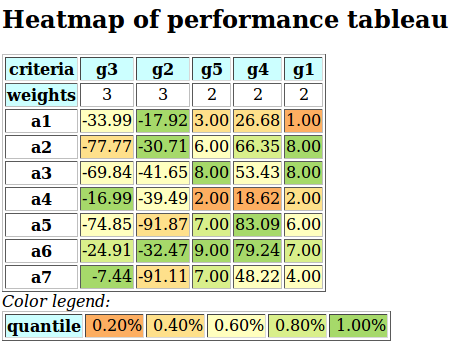
\includegraphics[width=10cm]{Figures/randomCBHeatmap.png}
\caption{Unordered heatmap of a random Cost-Benefit performance tableau}
\label{fig:6.2}       % Give a unique label
\end{figure}
 
Such a performance tableau may be stored and re-accessed as follows.
\begin{lstlisting}
>>> t.save('temp')
    *----- saving performance tableau in XMCDA 2.0 format  -------------*
    File: temp.py saved !
>>> from perfTabs import PerformanceTableau
>>> t = PerformanceTableau('temp')
\end{lstlisting}

\section{Random three objectives performance tableaux}
\label{sec:6.4}

We provide the \texttt{Random3ObjectivesPerformanceTableau} class\index{Random3ObjectivesPerformanceTableau@\texttt{Random3ObjectivesPerformanceTableau} class} for generating random performance tableaux concerning potential public policies evaluated with respect to three preferential decision objectives taking respectively into account \emph{economical}, \emph{societal} as well as \emph{environmental} aspects.

Each public policy is qualified randomly as performing \emph{weak} ($-$), \emph{fair} ($\sim$) or \emph{good} ($+$) on each of the three objectives. 
Generator directives are the following:
\begin{itemize}[leftmargin=0.5cm,rightmargin=0.5cm]
\item \texttt{numberOfActions} = $20$ (default), minimal number required is 3, 
\item \texttt{numberOfCriteria} = $13$ (default),
\item \texttt{weightDistribution} = \texttt{'equiobjectives'} (default) $|$ \\ \texttt{'random'} $|$ \texttt{'equisignificant'},
\item \texttt{weightScale} = (1,\texttt{numberOfCriteria}): only used when random criterion weights are requested,
\item \texttt{integerWeights} = \texttt{True} (default): \texttt{False} gives normalized rational weights, 
\item \texttt{commonScale} = ($0.0$,$100.0$),
\item \texttt{commonThresholds} = [$(5.0,0.0)$, $(10.0,0.0)$, $(60.0,0.0)$]: Performance discrimination thresholds may be set for \texttt{'ind'}, \texttt{'pref'} and \texttt{'veto'} thresholds,  
\item \texttt{commonMode} = [\texttt{'triangular'},\texttt{'variable'},$0.5$]: random number generators of various other types ('\emph{uniform}','\emph{beta}') are available. If the mode of the \texttt{'triangular'} distribution is set to \texttt{'variable'}, three modes at $0.3 (-)$, $0.5 (\sim)$, respectively $0.7 (+)$ of the common scale span are set at random for each coalition and action. 
\item \texttt{valueDigits} = 2 (default): evaluations are encoded as decimals,
\item \texttt{missingDataProbability} = $0.05$ (default): random insertion of missing values with given probability,  
\item \texttt{NA} := \texttt{Decimal} (default = $-999$); missing data symbol,
\item \texttt{seed} = \texttt{None} (default). 
\end{itemize}

\noindent \textbf{Example Python session:}
\begin{lstlisting}[caption={Generating a random 3 Objectives performance tableau},label=list:6.3]
>>> from randomPerfTabs import\
...            Random3ObjectivesPerformanceTableau
>>> t = Random3ObjectivesPerformanceTableau(\
...           numberOfActions=7,\
...           numberOfCriteria=13,\
...           weightDistribution='equiobjectives',\
...           seed=120)
>>> t.showObjectives()
  *------ show objectives -------"
   Eco: Economical aspect
    ec01 criterion of objective Eco 18
    ec05 criterion of objective Eco 18
    ec06 criterion of objective Eco 18
    ec12 criterion of objective Eco 18
    Total weight: 72.00 (4 criteria)
   Soc: Societal aspect
    so02 criterion of objective Soc 24
    so11 criterion of objective Soc 24
    so13 criterion of objective Soc 24
    Total weight: 72.00 (3 criteria)
   Env: Environmental aspect
    en03 criterion of objective Env 12
    en04 criterion of objective Env 12
    en07 criterion of objective Env 12
    en08 criterion of objective Env 12
    en09 criterion of objective Env 12
    en10 criterion of objective Env 12
    Total weight: 72.00 (6 criteria)
\end{lstlisting}
In Listing \ref{list:6.3} above, we notice that four \emph{equisignificant} criteria (\texttt{ec01}, \texttt{ec05}, \texttt{ec06}, and \texttt{ec12}) evaluate for instance the performance of the public policies from an \emph{economic} point of view (Lines 16-22). Three \emph{equisignificant} criteria do the same from a \emph{societal} (Lines 10-15), and six from an \emph{environmental} point of view (Lines 23-28). The '\texttt{equiobjectives}' directive results hence in a balanced total weight ($72.00$) for each decision objective. 

Variable \emph{triangular} modes ($0.3$, $0.5$ or $0.7$ of the span of the measure scale) for each objective result in a different performance status for each public policy with respect to the three objectives.
\begin{lstlisting}
>>> t.showActions()
  key:  p1
   short name:  p1
   name:       action p1 Eco- Soc+ Env+
   profile:    {'Eco':'weak', 'Soc':'good', 'Env':'good'}
  key:  p2
   short name:  p2
   name:       action p2 Eco- Soc- Env-
   profile:    {'Eco':'weak', 'Soc':'weak', 'Env':'weak'}
   ...
  key:  p7
   short name:  p7
   name:       action p7 Eco+ Soc- Env-
   profile:    {'Eco':'good', 'Soc':'weak', 'Env':'weak'}
\end{lstlisting}
Policy \texttt{p01}, for instance, will probably show \emph{good} performances wrt the \emph{societal} and \emph{environmental} aspects, and \emph{weak} performances wrt the \emph{economical} aspect, whereas policy p2 will probably appear among the potential worst choices.

We may inspect in Fig.~\ref{fig:6.3} the given random three-objectives performance tableau with the \texttt{showHTMPerformanceTableau()} method.
\begin{lstlisting}
>>> t.showHTMLPerformanceTableau()
\end{lstlisting}
\begin{figure}[h]
%\sidecaption[t]
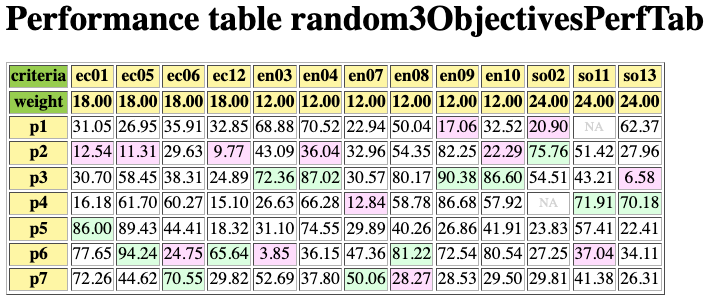
\includegraphics[width=12cm]{Figures/random3ObjPerfTab.png}
\caption{Browser view on the given random three-objectives performance tableau.}
\label{fig:6.3}       % Give a unique label
\end{figure}
Light green cells show best performances and light red worst performances. Policy \texttt{p01} shows thus the worst performance ($17.09/100.00$) on the environmental criterion \texttt{en09}, whereas policy \texttt{p03} shows the best performances on four out of the six \emph{environmental} criteria.

No trivial best choice becomes apparent when looking at the performance tableau shown in Fig.~\ref{fig:6.3}. Let us therefore compute a \Rubis best choice recommendation (see Chapter~\ref{sec:4}).
\begin{lstlisting}[caption={What is the public policy to recommend as best choice ?},label=list:6.4]
>>> from outrankingDigraphs import\
...       BipolarOutrankingDigraph
>>> g = BipolarOutrankingDigraph(t)
>>> g.showBestChoiceRecommendation()
  ***********************
  Rubis best choice recommendation(s) (BCR)
  (in decreasing order of determinateness)   
  Credibility domain: [-1.00,1.00]
  === >> potential best choice(s)
  * choice              : ['p3', 'p4', 'p5', 'p6']
   independence        : 0.00
   dominance           : 0.17
   absorbency          : -1.00
   covering (%)        : 41.67
   determinateness (%) : 52.98
   - most credible action(s) = { 'p3': 0.17, }
  === >> potential worst choice(s) 
  * choice              : ['p1', 'p2', 'p5', 'p7']
   independence        : 0.00
   dominance           : -0.44
   absorbency          : 0.19
   covered (%)         : 41.67
   determinateness (%) : 50.79
   - most credible action(s) = { 'p7': 0.06, }
\end{lstlisting}
Policy \texttt{p3} gives the most credible best choice candidate with the support of a $57.5\%$ majority of significance, whereas policy \texttt{p7} appears to be the less supported. Policy \texttt{p5} gives an ambiguous best and worst choice candidate. A drawing of the strict outranking digraph oriented by best and worst choices gives a more complete preferential picture (see Fig.~\ref{fig:6.4}).
\begin{lstlisting}
>>> (~(-g)).exportGraphViz(\
...             fileName='3ObjPerfTabBestChoice',\
...             bestChoice=['p3'],worstChoice=['p7'])
  *---- exporting a dot file for GraphViz tools ---------*
   Exporting to 3ObjPerfTabBestChoice.dot
   dot -Grankdir=BT -Tpng 3ObjPerfTabBestChoice.dot\
                    -o 3ObjPerfTabBestChoice.png
\end{lstlisting}
\begin{figure}[h]
\sidecaption[t]
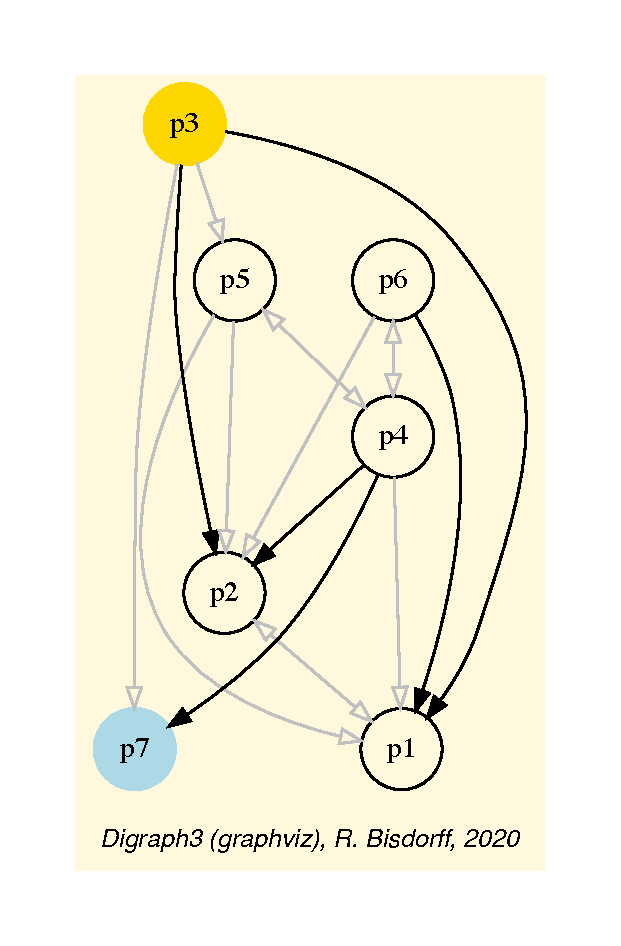
\includegraphics[width=6cm]{Figures/3ObjPerfTabBestChoice.pdf}
\caption{The strict outranking digraph oriented by best and worst choices. Policy \texttt{p5} is indeed incomparable --in a strict  outranking sense-- to all the other six policies. Policies \texttt{p1}, \texttt{p2} and \texttt{p7} appear strictly outranked.}
\label{fig:6.4}       % Give a unique label
\end{figure}

A heatmap view on the \Copeland ranked performance tableau confirms the best choice recommendation (see Section~\ref{sec:8.2}).
\begin{lstlisting}
>>> t.showHTMLPerformanceHeatmap(Correlations=True,\
...                        colorLevels=5,ndigits=1,\
...                        rankingRule='Copeland')
\end{lstlisting}
\begin{figure}[h]
%\sidecaption[t]
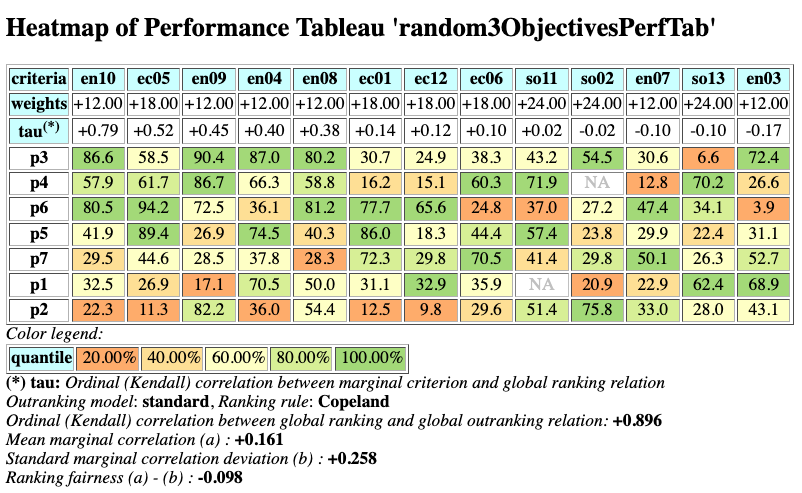
\includegraphics[width=12cm]{Figures/random3ObjHeatmap.png}
\caption{Browser view on the \Copeland ranked performance tableau.}
\label{fig:6.5}       % Give a unique label
\end{figure}
The heatmap view with its \Copeland ranking based on the bipolar outranking digraph confirms policy's \texttt{p3} as first-ranked. Notice also that the three strict outranked policies do effectively appear in the last positions. 
\clearpage
\section{Random academic performance tableaux}
\label{sec:6.5}

The \texttt{RandomAcademicPerformanceTableau} class\index{RandomAcademicPerformanceTableau@\texttt{RandomAcademicPerformanceTableau()}} constructor generates performance tableaux with random grades for a given number of students in different courses. 

\noindent Generator directives:
\begin{itemize}[leftmargin=0.5cm,rightmargin=0.5cm]
\item \texttt{numberOfStudents} := \texttt{Integer} (default 10)
\item \texttt{numberOfCourses} := \texttt{Integer} (default 5)
\item \texttt{weightDistribution} := '\emph{equisignificant}' | '\emph{random}' (default),
\item \texttt{weightScale} := $1$, $1$ - \texttt{numberOfCourses} (default when random)),
\item \texttt{IntegerWeights} := \texttt{Boolean} (True = default),
\item \texttt{commonScale} := (\texttt{Integer},\texttt{integer}) $(0,20)$ (default),
\item \texttt{ndigits} := \texttt{Integer} (default 0),
\item \texttt{WithTypes} := \texttt{Boolean} (default False),
\item \texttt{commonMode} := ('\emph{triangular}',$xm$=14,$r$=0.25) (default),
\item \texttt{commonThresholds} := {'ind':(0,0), 'pref':(1,0)} (default),
\item \texttt{missingDataProbability} := 0.0 (default),
\item \texttt{NA} := \texttt{Decimal} (default = $-999$); missing data symbol. 
\end{itemize}      

When Parameter \texttt{WithTypes} is set to \texttt{True}, the students are randomly allocated to one of the following four categories --\emph{weak} (1/6), \emph{fair} (1/3), \emph{good} (1/3), and \emph{excellent} (1/3)-- in the bracketed proportions. In a default $0-20$ grading range, the random range of a weak student is $0-10$, of a fair student $4-16$, of a good student $8-20$, and of an excellent student $12-20$. The random grading generator follows in this case a double triangular probablity law with \emph{mode} ($xm$) equal to the middle of the random range and median repartition ($r = 0.5$) of probability each side of the mode.
\begin{lstlisting}[caption={Generating a random academic performance tableau},label=list:6.5]
>>> from randomPerfTabs import RandomAcademicPerformanceTableau
>>> t = RandomAcademicPerformanceTableau(\
...        numberOfStudents=11,\
...        numberOfCourses=7, missingDataProbability=0.03,\
...        WithTypes=True, seed=100)
>>> t
  *------- PerformanceTableau instance description ------*
   Instance class   : RandomAcademicPerformanceTableau
   Seed             : 100
   Instance name    : randstudPerf
   Actions          : 11
   Criteria         : 7
   NA proportion(%) : 5.2
   Attributes       : ['randomSeed', 'name', 'actions',
             'criteria', 'evaluation', 'weightPreorder']
>>> t.showPerformanceTableau()
  *----  performance tableau -----*
   Courses |   'm1'  'm2'  'm3'  'm4'  'm5'  'm6'  'm7' 
     ECTS  |    2     1     3     4     1     1     5    
  ---------|------------------------------------------
    's01f' |    12    13    15    08    16    06    15   
    's02g' |    10    15    20    11    14    15    18   
    's03g' |    14    12    19    11    15    13    11   
    's04f' |    13    15    12    13    13    10    06   
    's05e' |    12    14    13    16    15    12    16   
    's06g' |    17    13    10    14    NA    15    13   
    's07e' |    12    12    12    18    NA    13    17   
    's08f' |    14    12    09    13    13    15    12   
    's09g' |    19    14    15    13    09    13    16   
    's10g' |    10    12    14    17    12    16    09   
    's11w' |    10    10    NA    10    10    NA    08
>>> t.weightPreorder
  [['m2', 'm5', 'm6'], ['m1'], ['m3'], ['m4'], ['m7']]
\end{lstlisting}
  
The example tableau, generated for instance above with \texttt{missingDataProbability} = $0.03$, \texttt{WithTypes} = \texttt{True} and \texttt{seed} = 100 (see Listing \ref{list:6.5} Lines 2-5), results in a set of two excellent (\texttt{s05e} and \texttt{s07e}), five good (\texttt{s02g}, \texttt{s03g}, \texttt{s06g}, \texttt{s09g} and \texttt{s10g}), three fair (\texttt{s01f}, \texttt{s04f} and \texttt{s08f}) and one weak (\texttt{s11w}) students. Notice that six students get a grade below the course validating threshold of $10$ and we observe four missing grades (\texttt{NA}), two in course \texttt{m5} and, one in courses \texttt{m3} and \texttt{m6} (see Lines 20-30).

A statistical summary of the students' grades obtained in the heighest weighted course, namely \texttt{m7}, is shown with the \texttt{showCourseStatistics()} method. \index{showCourseStatistics@\texttt{showCourseStatistics()}}
\begin{lstlisting}[caption={Student performance summary statistics per course},label=list:6.6]
>>> t.showCourseStatistics('m7')
  *----- Summary performance statistics ------*
   Course name    : m7
   Course weight  : 5
   Students       : 11
   Grading scale  : 0.00 - 20.00
   Missing evaluations : 0
   Mean evaluation       : 12.82
   Standard deviation    : 3.79
   Maximal evaluation    : 18.00
   Quantile Q3 (x_75)    : 16.25
   Median evaluation     : 14.00
   Quantile Q1 (x_25)    : 10.50
   Minimal evaluation    : 6.00
   Mean absolute difference      : 4.30
   Standard difference deviation : 5.35
\end{lstlisting}
In Listing~\ref{list:6.6}, the Course \texttt{m7} evaluation statistics show a mean grade of $12.82$ and a median grade of $14$. Maximal (resp. minimal) grade is $18$ (resp. $6$).

With a ranked heatmap view on all the grades we get a global pictures of the performance of all the eleven students. 
\begin{figure}[h]
%\sidecaption[t]
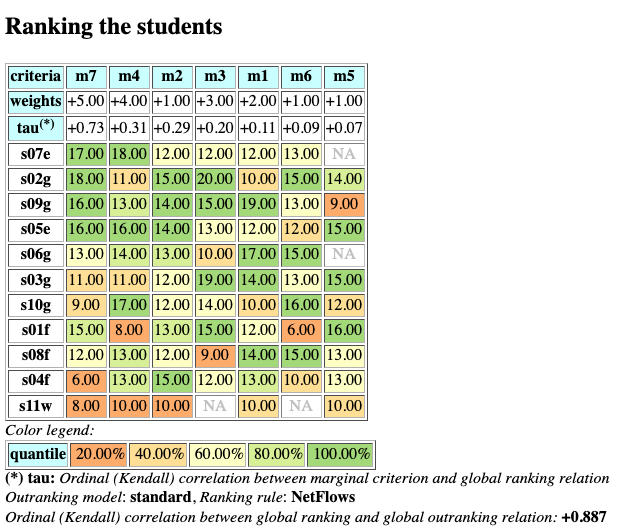
\includegraphics[width=12cm]{Figures/rankingStudents.png}
\caption{Ranking the students in a performance heatmap view.}
\label{fig:6.6}       % Give a unique label
\end{figure}
The ranking shown here in Fig.~\ref{fig:6.6}, produced with the \NetFlows ranking rule (see Section~\ref{sec:8.3}), reports a high correlation of $+0.887$ with the corresponding bipolar-valued outranking digraph (see Section~\ref{sec:8.3}).

The \NetFlows ranking represents also a rather \emph{fair weighted consensus} between the individual courses' marginal rankings as made apparent in Listing~\ref{list:6.7} below with the \texttt{showRankingConsensusQuality()} method. \index{showRankingConsensusQuality@\texttt{showRankingConsensusQuality()}}
\begin{lstlisting}[caption={Consensus quality of the students's ranking},label=list:6.7]
>>> from outrankingDigraphs import\
...                  BipolarOutrankingDigraph
>>> g = BipolarOutrankingDigraph(t)
>>> t.showRankingConsensusQuality(\
...                 g.computeNetFlowsRanking())
  Consensus quality of ranking:
  ['s07', 's02', 's09', 's05', 's06', 's03', 's10',
   's01', 's08', 's04', 's11']
  Criterion (weight): correlation
  -------------------------------
     'm7' (0.294): +0.727
     'm4' (0.235): +0.309
     'm2' (0.059): +0.291
     'm3' (0.176): +0.200
     'm1' (0.118): +0.109
     'm6' (0.059): +0.091
     'm5' (0.059): +0.073
  Summary:
   Weighted mean marginal correlation (a): +0.361
   Standard deviation (b)                : +0.248
   Ranking fairness (a)-(b)              : +0.113
\end{lstlisting}
The correlation with the marginal course rankings follows precisely the given ECTS weights. Course \texttt{m7}, with the highest relative weight ($0.294$) is most present ($+0.727$) in the global \NetFlows ranking and no course marginal ranking appears negatively correlated with this ranking. The mean weighted correlation is $+0.361$.

\vspace{1cm}
Useful multiple incommensuarble criteria ranking rules are presented and discussed in detail in Chapter~\ref{sec:8}. In the next Chapter~\ref{sec:7}, we first show how to compute the winner of an election on the basis of a different performance evaluation model, namely \emph{linear voting profiles} who are discussed in social choice theory.